% 第1章 立论依据

\chapter{一、立论依据}

\section{（1）课题来源、选题依据和立论背景}

本课题围绕发动机燃烧场多组分浓度与关键自由基二维分布的同步诊断这一核心科学问题展开。

一氧化氮（NO）是燃烧排放中危害最大、也最难控制的痕量污染物之一：它既是光化学烟雾、酸雨与臭氧层消耗的前体，又是燃烧组织优劣与排放合规程度的直接指示物。在航空发动机、燃气轮机、工业炉窑等实际燃烧装置中，NO 的排放控制长期面临一个共性难题——``看不见、量不准''：火焰内部 NO 的时空分布与绝对浓度难以同步获得，导致减排措施缺乏可靠的定量依据。这一困境具体表现在三个层面：其一，NO 生成机理交织，仿真难以单独支撑。NO 主要通过热力型（Zeldovich 机理，高温区主导）、快速型（Fenimore 机理，火焰前沿）与燃料型（含氮燃料氧化）三条途径生成，其对温度、当量比、停留时间的依赖截然不同，仅靠数值仿真难以准确预测工程装置中的 NO 生成，必须有高时空分辨的实验测量进行判别与验证。其二，传统测量手段难以胜任原位测量。取样法（化学发光、气相色谱）需将气体抽出，破坏流场且响应慢，无法反映瞬态分布；接触式电化学传感器无法承受高温火焰环境，使火焰内部 NO 的分布长期处于``测不到''的状态。其三，现有激光诊断手段各有短板，单一方法难以兼顾成像与定量：激光诱导荧光（PLIF）能给出二维 NO 分布图像，但定量化受荧光猝灭、温度依赖与激光能量衰减等因素制约，标定困难；可调谐激光吸收光谱（TDLAS）能免标定地给出绝对浓度，但只能做视线路径上的积分测量，无法获得空间分布。单一手段始终难以同时满足``看得见''与``量得准''的双重要求，不同系统之间也缺乏可溯源、可相互验证的统一基准。

随着航空发动机、燃气轮机等动力装备向高推重比、低排放方向发展，燃烧室内部温度、组分浓度与反应区结构的精确表征成为燃烧组织优化与排放控制的关键。然而，发动机燃烧场具有高温（可达 2000 K 以上）、高速（湍流脉动微秒量级）、强梯度与强干扰（H$_2$O/CO$_2$ 大量存在）等特征，传统接触式探针（热电偶、取样分析）受响应速度、侵入扰动与寿命限制，难以满足瞬态、非接触、多参数同步测量的要求。激光吸收光谱（TDLAS）与平面激光诱导荧光（PLIF）是当前最具代表性的两类非接触光学诊断手段：前者以高灵敏度、高精度、可定量著称，适合组分浓度与温度的``线/点''测量；后者以高时空分辨、可成场著称，适合火焰结构与自由基``面''分布的瞬态捕捉。二者互补，但受限于可调谐激光器波段覆盖与高能高频光源的可获得性，实现``同一燃烧场内多组分浓度 + 关键自由基分布''的同步测量仍是难点。正是针对上述困境，本课题提出``成像与定量互补、相互验证''的研究思路：以染料激光倍频产生 283 nm 紫外光实现 NO-PLIF 二维成像，以中红外量子级联激光实现 NO 绝对浓度的 TDLAS 定量，二者围绕同一火焰对象交叉标定，建立可溯源的 NO 测量与标定体系。本课题正是基于课题组已有的中红外量子级联激光器（QCL）多通道平台与高频 burst 染料激光平台，围绕上述难点展开，选题具有明确的应用牵引与理论探索价值。

\begin{figure}[H]
  \centering
  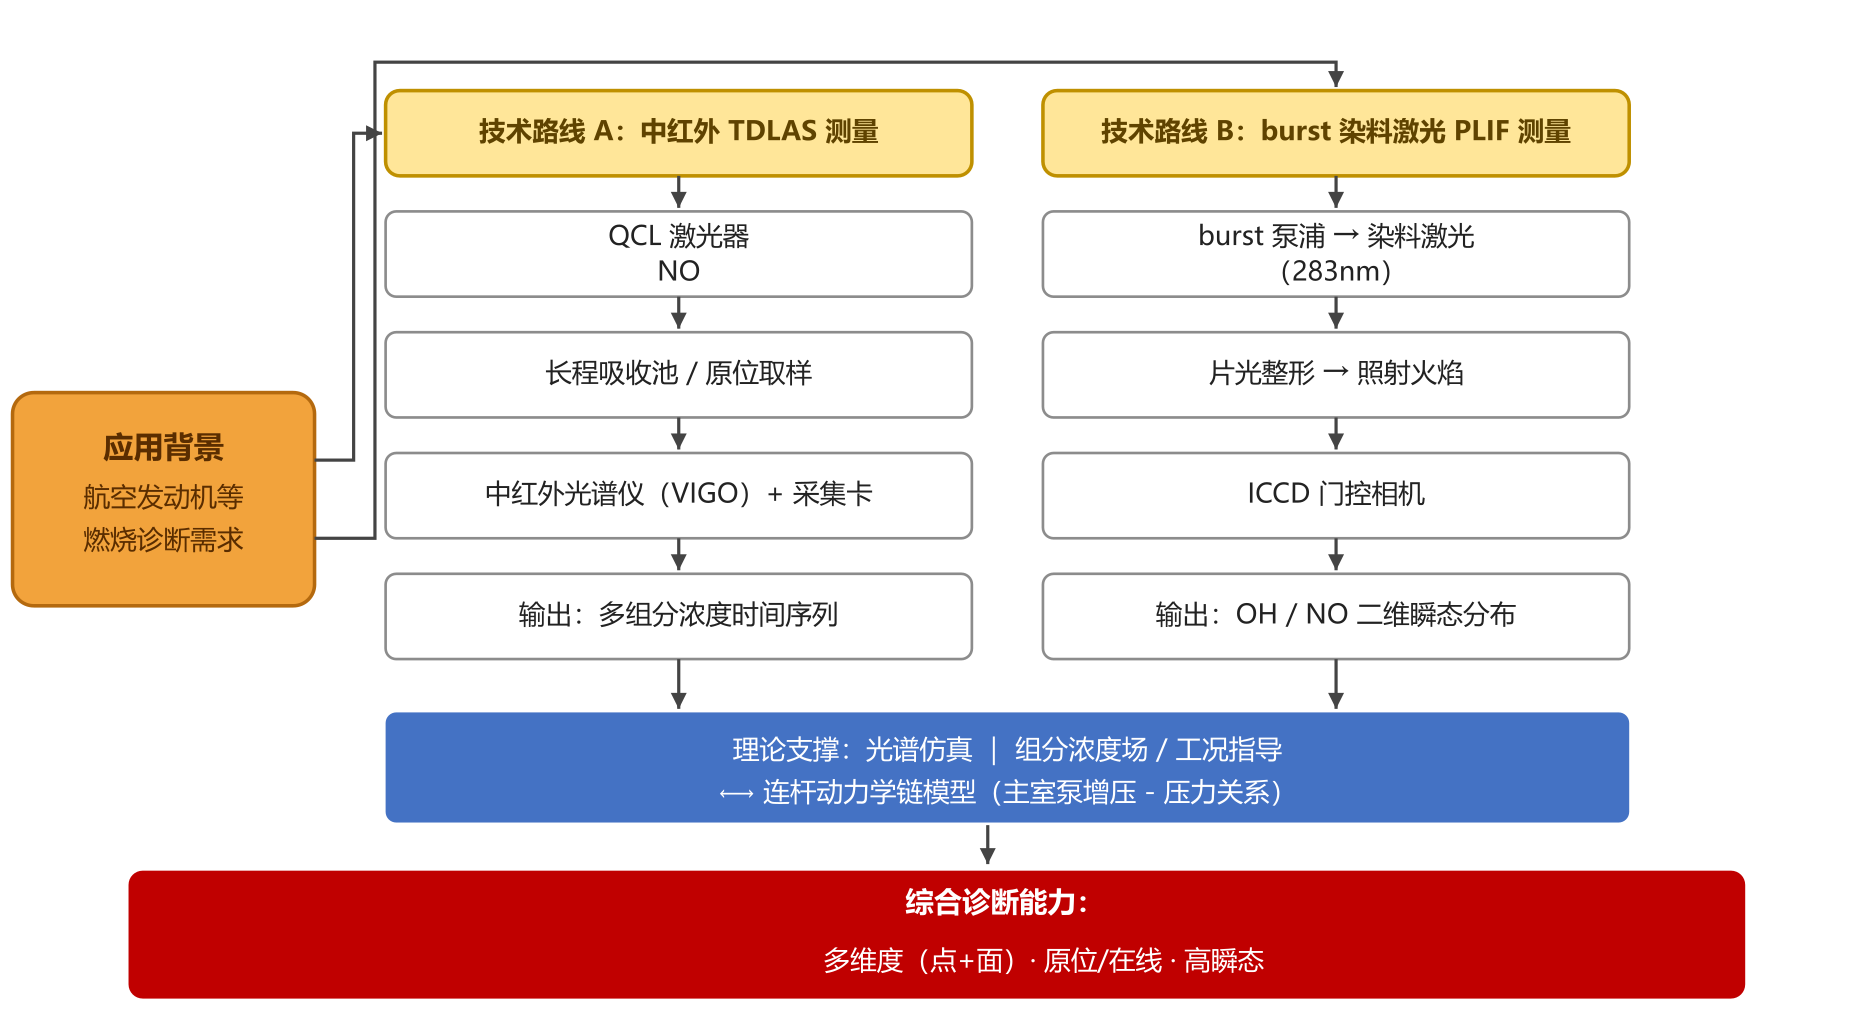
\includegraphics[width=0.85\textwidth]{figures/image1.png}
  \caption{课题总体技术框架：中红外 TDLAS 多组分线测量与 burst 染料激光 NO-PLIF 面测量的协同}
  \label{fig:framework}
\end{figure}

\section{二、课题研究目的、理论意义和实际应用价值}

\subsection{（1）课题研究目的}

本课题以发动机尾气/燃烧场中 NO 的高保真在线诊断与多组分同步诊断为总目标，围绕``定量测量 $\rightarrow$ 二维成像 $\rightarrow$ 手段互校验''三条技术线展开，具体研究目的如下：

（1）建立中红外 QCL-TDLAS 的 NO 在线定量测量方法与浓度反演模型，并同步拓展 CO 通道。面向 NO 5.2 μm 基频带（约 1876 cm$^{-1}$）与 CO 4.6 μm 基频带（约 2143 cm$^{-1}$），开展高温、高压、多组分干扰下的特征谱线筛选与干扰抑制研究；建立基于 Voigt 线型的``吸收谱—温度—浓度''联合反演模型，厘清谱线强度、配分函数、压力展宽与基线抖动等因素对反演误差的传递规律，实现 NO（及同步 CO）浓度的在线、定量、免标定反演。

（2）建立 burst 染料激光泵浦的 NO-PLIF 二维瞬态成像系统，并实现稳定出光与标定。利用 burst 模式染料激光输出 283 nm（NO A$^2\Sigma^+ \leftarrow X^2\Pi$ (0,0) 跃迁）激发 NO 荧光，构建高频脉冲串泵浦的 NO-PLIF 成像光路；攻克染料激光在 burst 模式下的能量稳定性、线宽压窄与频率锁定等关键问题；完成系统的强度—浓度标定，实现 NO 二维浓度场的瞬态、高帧频成像。

（3）探明 QCL-TDLAS 与 NO-PLIF 两种手段在发动机尾气工况下的耦合与互校验机制，形成一体化诊断能力。以 NO 为主线：用 NO-PLIF 的二维分布为 TDLAS 的路径积分反演提供空间均匀性先验、校正``路径平均浓度''与``峰值浓度''的差异；用 TDLAS 的定量浓度反演结果反向校准 NO-PLIF 的强度—浓度标定；建立两者的互校验模型与不确定度传递框架，最终形成``线定量 + 场成像''相互印证的一体化 NO 诊断平台。

\subsection{（2）理论意义}

其一，揭示``线定量—场成像''互补诊断的物理与信息学基础，阐明路径积分浓度与二维浓度场之间的空间映射与权重构造关系，为多手段协同诊断提供理论框架。其二，建立多组分吸收谱（TDLAS）与自由基荧光图像（PLIF）在标准火焰场下的联合标定理论，发展碰撞猝灭、温度—组分依赖与激发效率的统一校正方法。其三，发展高重频 burst 染料激光``高压染料循环稳流 + 蓄能缓冲''的稳定性控制理论，揭示汽蚀抑制、流场均匀性与输出能量抖动的关联机制。其四，构建双向互校验模型与合成不确定度传递框架，推动燃烧激光诊断由``单点/单法''向``可溯源、可互校''演进。

\subsection{（3）实际应用价值}

本课题成果可直接服务于航空发动机、燃气轮机、工业炉窑等动力与能源装备的低排放燃烧组织与 NOx 排放合规：提供可溯源的 NO 在线诊断手段，使减排措施获得可靠的定量依据。所形成的一体化``线定量 + 场成像''诊断能力，可推广至 CO、CO$_2$、N$_2$O 等多组分与 OH 等关键自由基的同步诊断；所搭建的中红外 QCL-TDLAS 与高频 burst 染料激光 PLIF 两套平台，亦可辐射至燃烧、流体与等离子体诊断等相关研究，具有重要的工程应用前景。
